\clearpage
\section*{PHỤ LỤC G. PHÂN RÃ CHỨC NĂNG CHI TIẾT}
\phantomsection\addcontentsline{toc}{section}{PHỤ LỤC G. PHÂN RÃ CHỨC NĂNG CHI TIẾT}
\label{app:chapter2-details}
\setcounter{figure}{0}\renewcommand{\thefigure}{G.\arabic{figure}}
Các nhóm chức năng dưới đây triển khai chi tiết từ sơ đồ tổng quát ở Chương 2. Mỗi nhóm gắn với một phạm vi nghiệp vụ; các bước dùng chung được giữ trong cùng nhóm để thể hiện trách nhiệm xử lý.

\clearpage
Nhóm tài khoản quản lý đăng nhập, đăng ký, khôi phục mật khẩu và phiên truy cập theo vai trò.
\begin{figure}[H]\centering
\includegraphics[page=2,width=\textwidth,height=0.78\textheight,keepaspectratio]{chapter2/usecase_decomposition_v2.pdf}
\caption{Phân rã chức năng: tài khoản và phiên.}\label{fig:app-functions-2}
\end{figure}

\clearpage
Khám phá không gian kết hợp tìm kiếm, bộ lọc, bản đồ và thông tin phòng trước khi đặt.
\begin{figure}[H]\centering
\includegraphics[page=3,width=\textwidth,height=0.78\textheight,keepaspectratio]{chapter2/usecase_decomposition_v2.pdf}
\caption{Phân rã chức năng: khám phá không gian.}\label{fig:app-functions-3}
\end{figure}

\clearpage
Yêu cầu đặt chỗ bao gồm chọn kỳ thuê, kiểm tra khả dụng, chốt giá và mở QR với thời hạn giữ lịch tạm.
\begin{figure}[H]\centering
\includegraphics[page=4,width=\textwidth,height=0.78\textheight,keepaspectratio]{chapter2/usecase_decomposition_v2.pdf}
\caption{Phân rã chức năng: tạo yêu cầu đặt chỗ.}\label{fig:app-functions-4}
\end{figure}

\clearpage
Theo dõi lượt thuê phân biệt lịch sử, thời hạn thanh toán và điều kiện hủy; nhả lịch đi cùng cập nhật trạng thái.
\begin{figure}[H]\centering
\includegraphics[page=5,width=\textwidth,height=0.78\textheight,keepaspectratio]{chapter2/usecase_decomposition_v2.pdf}
\caption{Phân rã chức năng: lịch đặt và hủy.}\label{fig:app-functions-5}
\end{figure}

\clearpage
Hồ sơ Host được xét duyệt riêng với minh chứng vị trí hoặc hình ảnh của tài sản.
\begin{figure}[H]\centering
\includegraphics[page=6,width=\textwidth,height=0.78\textheight,keepaspectratio]{chapter2/usecase_decomposition_v2.pdf}
\caption{Phân rã chức năng: hồ sơ host và xác minh.}\label{fig:app-functions-6}
\end{figure}

\clearpage
Quản lý tài sản tách tòa nhà, phòng, cấu hình giá và lịch; công bố phòng phụ thuộc trạng thái xét duyệt và hoạt động.
\begin{figure}[H]\centering
\includegraphics[page=7,width=\textwidth,height=0.78\textheight,keepaspectratio]{chapter2/usecase_decomposition_v2.pdf}
\caption{Phân rã chức năng: quản lý không gian.}\label{fig:app-functions-7}
\end{figure}

\clearpage
Vận hành lượt thuê phân biệt nhận phòng, hoàn tất và không đến, không suy ra đã sử dụng chỉ từ thời gian.
\begin{figure}[H]\centering
\includegraphics[page=8,width=\textwidth,height=0.78\textheight,keepaspectratio]{chapter2/usecase_decomposition_v2.pdf}
\caption{Phân rã chức năng: theo dõi và sử dụng.}\label{fig:app-functions-8}
\end{figure}

\clearpage
Chat gắn với cặp thành viên, cập nhật tin cuối và mốc đọc; liên hệ không cấp quyền đọc hội thoại cho bên ngoài.
\begin{figure}[H]\centering
\includegraphics[page=9,width=\textwidth,height=0.78\textheight,keepaspectratio]{chapter2/usecase_decomposition_v2.pdf}
\caption{Phân rã chức năng: chat và liên hệ.}\label{fig:app-functions-9}
\end{figure}

\clearpage
Đánh giá chỉ gắn với lượt đã khép và có xác nhận sử dụng, nhằm tách trải nghiệm thật khỏi lượt không đến.
\begin{figure}[H]\centering
\includegraphics[page=10,width=\textwidth,height=0.78\textheight,keepaspectratio]{chapter2/usecase_decomposition_v2.pdf}
\caption{Phân rã chức năng: đánh giá sau sử dụng.}\label{fig:app-functions-10}
\end{figure}

\clearpage
Báo cáo là hồ sơ xử lý vi phạm có phản hồi của Host và kết luận của Admin, tách với nội dung đánh giá.
\begin{figure}[H]\centering
\includegraphics[page=11,width=\textwidth,height=0.78\textheight,keepaspectratio]{chapter2/usecase_decomposition_v2.pdf}
\caption{Phân rã chức năng: báo cáo và phản hồi.}\label{fig:app-functions-11}
\end{figure}

\clearpage
Quản trị bao gồm kiểm duyệt, hạn chế hoạt động và xử lý từng ngoại lệ của booking, có lưu lý do.
\begin{figure}[H]\centering
\includegraphics[page=12,width=\textwidth,height=0.78\textheight,keepaspectratio]{chapter2/usecase_decomposition_v2.pdf}
\caption{Phân rã chức năng: quản trị và sự cố.}\label{fig:app-functions-12}
\end{figure}

\clearpage
Theo dõi và nhật ký phục vụ đối chiếu thay đổi; bộ đếm và lịch giữ chỗ phải khớp với các booking đang hiệu lực.
\begin{figure}[H]\centering
\includegraphics[page=13,width=\textwidth,height=0.78\textheight,keepaspectratio]{chapter2/usecase_decomposition_v2.pdf}
\caption{Phân rã chức năng: theo dõi và nhật ký.}\label{fig:app-functions-13}
\end{figure}

\clearpage
Hồ sơ và thông báo tổng hợp thông tin cá nhân, ảnh đại diện và các cập nhật liên quan đến tài khoản.
\begin{figure}[H]\centering
\includegraphics[page=14,width=\textwidth,height=0.78\textheight,keepaspectratio]{chapter2/usecase_decomposition_v2.pdf}
\caption{Phân rã chức năng: hồ sơ và thông báo.}\label{fig:app-functions-14}
\end{figure}

\clearpage
Thanh toán demo dùng một kênh payOS: tạo QR, đối soát nhận tiền và cập nhật kết quả; không tự hoàn tiền.
\begin{figure}[H]\centering
\includegraphics[page=15,width=\textwidth,height=0.78\textheight,keepaspectratio]{chapter2/usecase_decomposition_v2.pdf}
\caption{Phân rã chức năng: thanh toán demo.}\label{fig:app-functions-15}
\end{figure}
